\documentclass[11pt, a4paper,twocolumn]{jarticle}
\usepackage[dvipdfmx]{graphicx}
\usepackage{listings,jlisting}

\begin{document}
%=============================================================
\section{一次元走査光学系の特性評価}
\subsection{目的}
正弦波変調パターンを測定することにより,構成した光学系の特性を評価する.

\subsection{手順}
まず図\ref{fig:10}に示すような正弦波変調パターン画像を入力物体として用いた. \\

\noindent
\textbf{9-1} \\
周期2.0mmパターンのサンプルを用いて表\ref{fig:foo}のように異なる走査ピッチ(サンプリング間隔)で測定を行った. \\

\noindent
\textbf{9-2} \\
データ数2500,サンプリング周波数500に固定し,\ref{fig:foofoo}のようにパターンの周期を変えながら画像データを取得しそのコントラストを求めた. \\

\noindent
\textbf{9-3} \\
物体を光軸と垂直方向にシフトさせ,集光スポットが楕円形になった状態から計測を開始し,2と同様に測定を行った.
この際,データ数2500,サンプリング周波数500に固定し,0.4mm,0.6mmのパターン周期での測定は省略した.

\begin{table}[ht]
\centering
\caption{実験9-1}
\begin{tabular}{c c c}
\hline
 & データ数 & サンプリング周波数[Hz] \\ \hline
9-1-1 & 10000 & 1000 \\
9-1-2 & 5000 & 500 \\
9-1-3 & 1000 & 100 \\
9-1-4 & 100 & 10 \\
9-1-5 & 10 & 1 \\
\end{tabular}
\label{fig:foo}
\end{table}

\begin{table}[ht]
\centering
\caption{実験9-2}
\begin{tabular}{c c}
\hline
 & パターン周期[mm]\\ \hline
9-2-1 & 0.4 \\
9-2-2 & 0.6 \\
9-2-3 & 1.0 \\
9-2-4 & 1.5 \\
9-2-5 & 2.0 \\
9-2-6 & 2.5 \\
\end{tabular}
\label{fig:foofoo}
\end{table}

\begin{figure}[ht]
 \begin{center}
  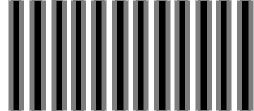
\includegraphics[width=0.8\linewidth]{fig10.png}
 \end{center}
 \caption{正弦波変調パターン}
 \label{fig:10}
\end{figure}

\subsection{結果}
\noindent
\textbf{9-1} \\
測定の結果以下のようなグラフが得られた.

\begin{figure}[ht]
 \begin{center}
  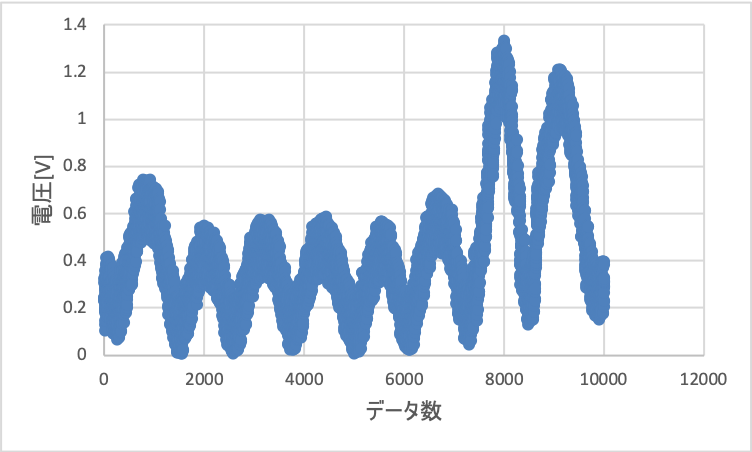
\includegraphics[width=0.8\linewidth]{fig11.png}
 \end{center}
 \caption{9-1-1}
 \label{fig:11}
\end{figure}

\begin{figure}[ht]
 \begin{center}
  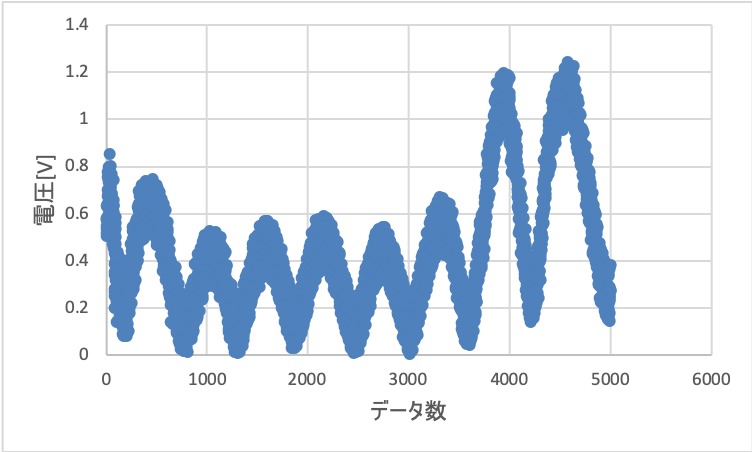
\includegraphics[width=0.8\linewidth]{fig12.png}
 \end{center}
 \caption{9-1-2}
 \label{fig:12}
\end{figure}

\begin{figure}[ht]
 \begin{center}
  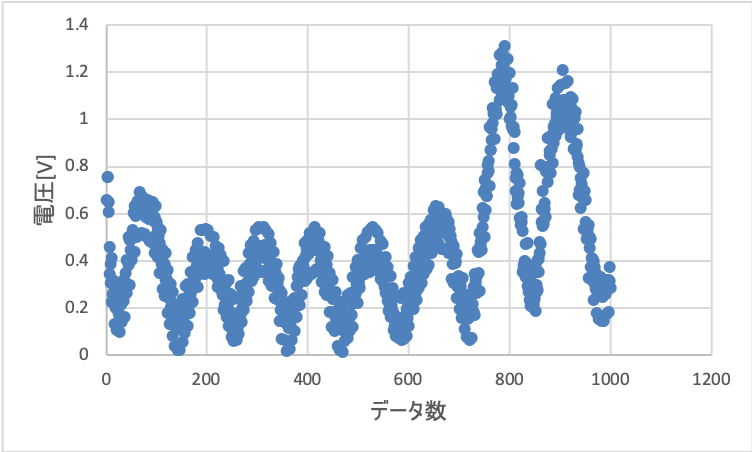
\includegraphics[width=0.8\linewidth]{fig13.png}
 \end{center}
 \caption{9-1-3}
 \label{fig:13}
\end{figure}

\begin{figure}[ht]
 \begin{center}
  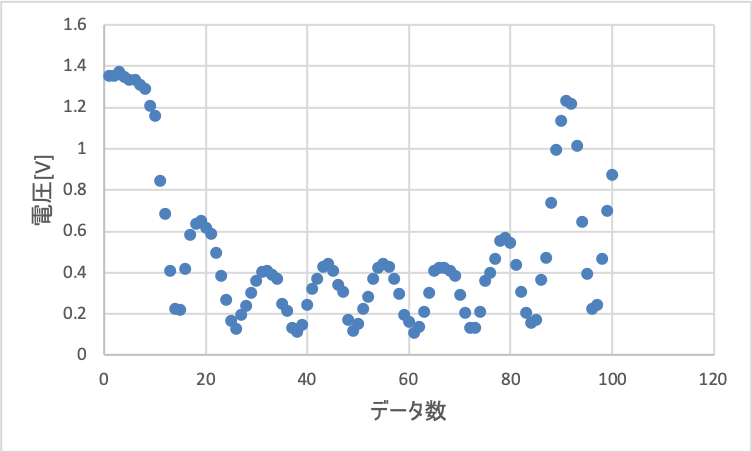
\includegraphics[width=0.8\linewidth]{fig14.png}
 \end{center}
 \caption{9-1-4}
 \label{fig:14}
\end{figure}

\begin{figure}[ht]
 \begin{center}
  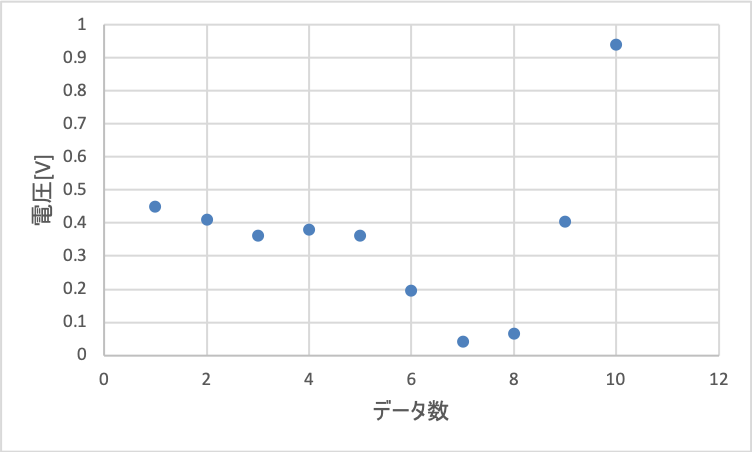
\includegraphics[width=0.8\linewidth]{fig15.png}
 \end{center}
 \caption{9-1-5}
 \label{fig:15}
\end{figure}

\noindent
\textbf{9-2} \\
測定の結果以下のようなグラフが得られた.

\begin{figure}[ht]
 \begin{center}
  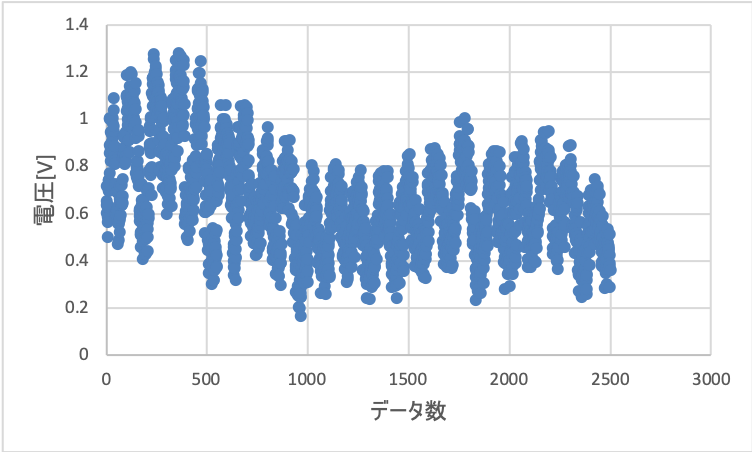
\includegraphics[width=0.8\linewidth]{fig16.png}
 \end{center}
 \caption{9-2-1}
 \label{fig:16}
\end{figure}

\begin{figure}[ht]
 \begin{center}
  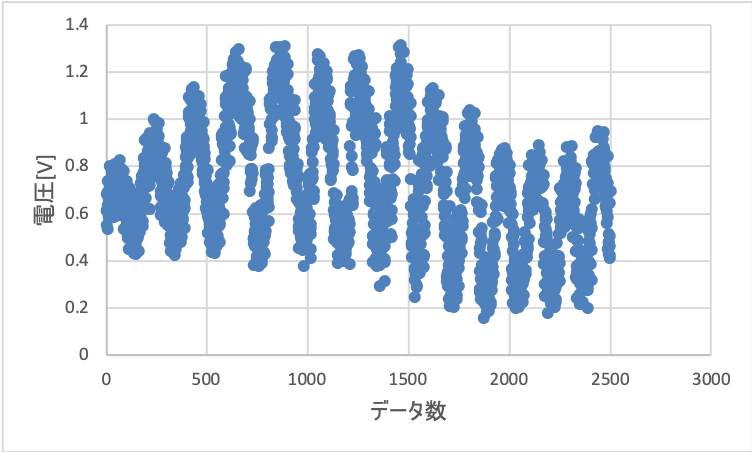
\includegraphics[width=0.8\linewidth]{fig17.png}
 \end{center}
 \caption{9-2-2}
 \label{fig:17}
\end{figure}

\begin{figure}[ht]
 \begin{center}
  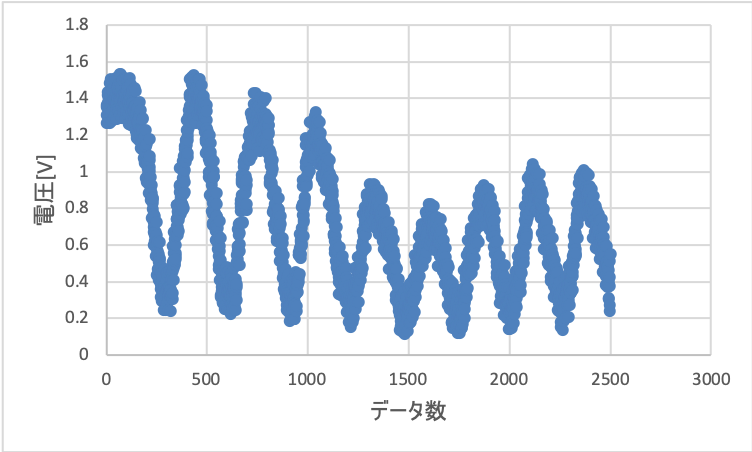
\includegraphics[width=0.8\linewidth]{fig18.png}
 \end{center}
 \caption{9-2-3}
 \label{fig:18}
\end{figure}

\begin{figure}[ht]
 \begin{center}
  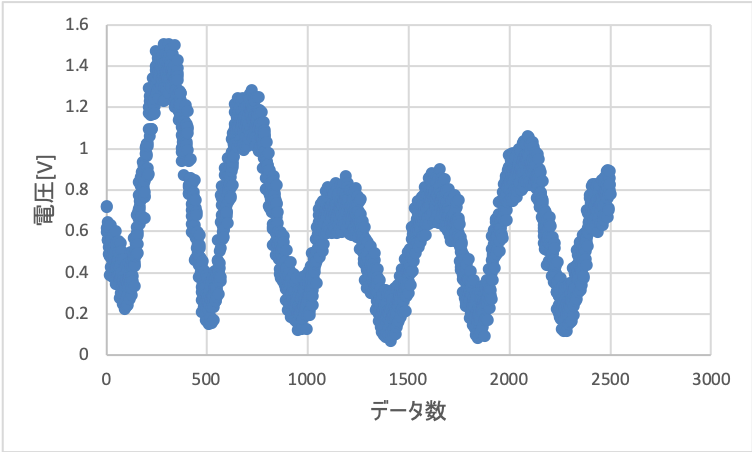
\includegraphics[width=0.8\linewidth]{fig19.png}
 \end{center}
 \caption{9-2-4}
 \label{fig:19}
\end{figure}

\begin{figure}[ht]
 \begin{center}
  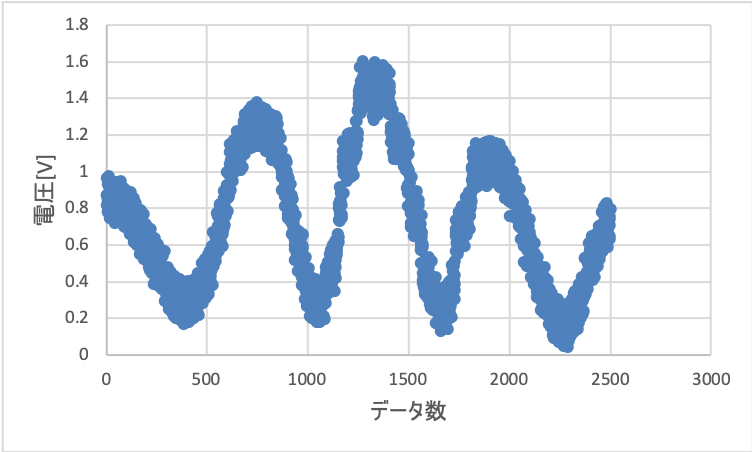
\includegraphics[width=0.8\linewidth]{fig20.png}
 \end{center}
 \caption{9-2-5}
 \label{fig:20}
\end{figure}

\begin{figure}[ht]
 \begin{center}
  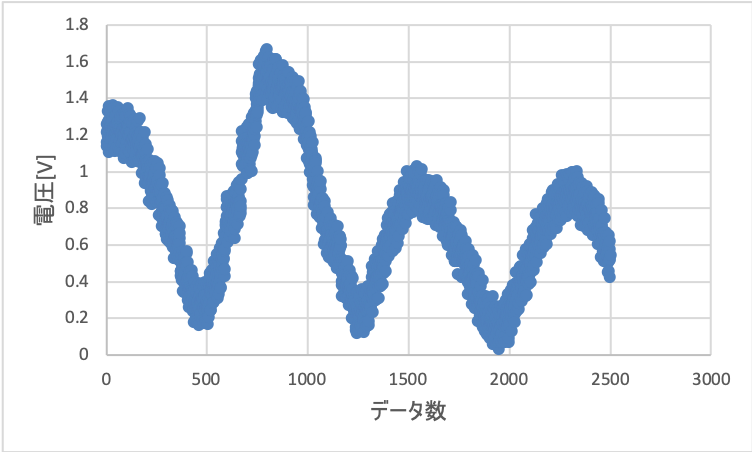
\includegraphics[width=0.8\linewidth]{fig21.png}
 \end{center}
 \caption{9-2-6}
 \label{fig:21}
\end{figure}

\noindent
\textbf{9-3} \\
測定の結果以下のようなグラフが得られた.

\begin{figure}[ht]
 \begin{center}
  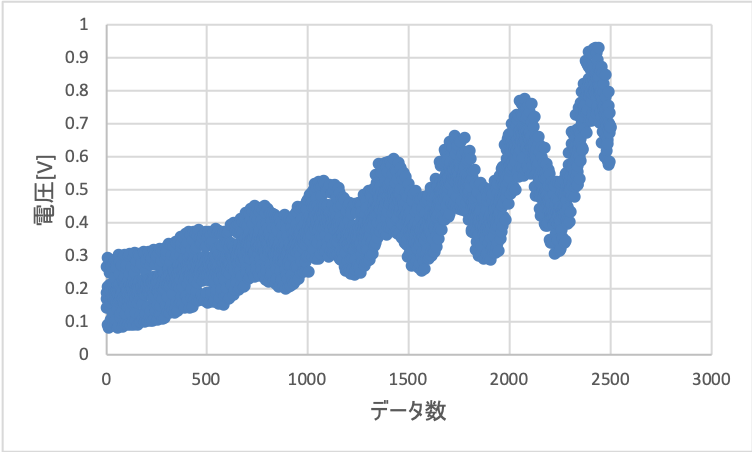
\includegraphics[width=0.8\linewidth]{fig22.png}
 \end{center}
 \caption{9-3-1}
 \label{fig:22}
\end{figure}

\begin{figure}[ht]
 \begin{center}
  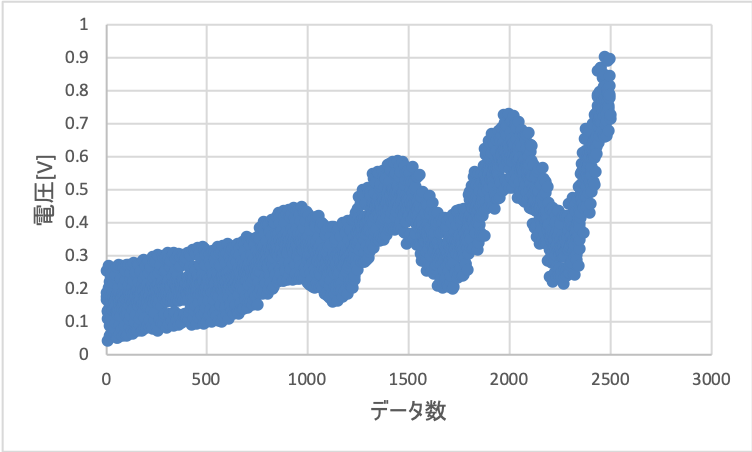
\includegraphics[width=0.8\linewidth]{fig23.png}
 \end{center}
 \caption{9-3-2}
 \label{fig:23}
\end{figure}

\begin{figure}[ht]
 \begin{center}
  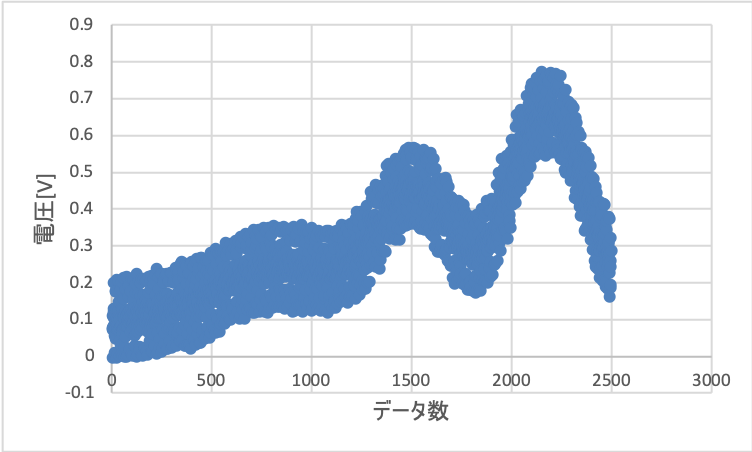
\includegraphics[width=0.8\linewidth]{fig24.png}
 \end{center}
 \caption{9-3-3}
 \label{fig:24}
\end{figure}

\begin{figure}[ht]
 \begin{center}
  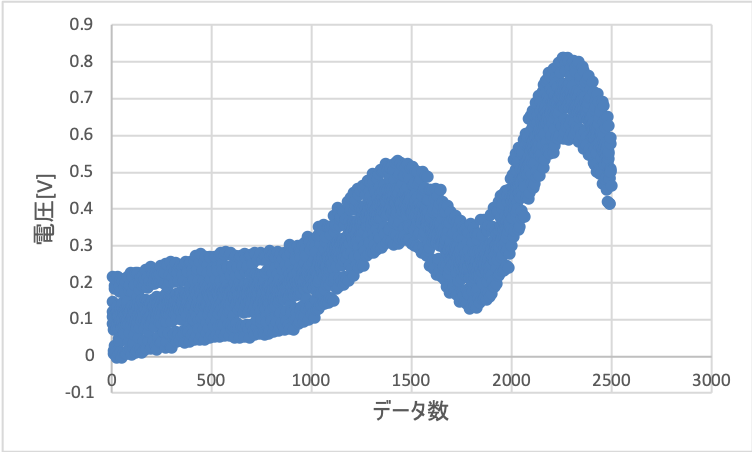
\includegraphics[width=0.8\linewidth]{fig25.png}
 \end{center}
 \caption{9-3-4}
 \label{fig:25}
\end{figure}

\clearpage

\subsection{考察}
まず実験9-1においては図\ref{fig:14}まではパターン周期と同じように測定できている一方で図\ref{fig:15}においては測定対象の周期を正確に読み取れていないため,走査ピッチが大きすぎたことによるエリアシングが起きたと考えられる.
サンプリング定理よりサンプリング周波数はは測定対象のパターン周波数の2倍より多くとっておく必要があると予測される.
実験9-2においては0.2mmのサンプルに対しても正確な測定を行うことができたのでこの光学系の分解能は0.2mm以上であることが予想される.
ここで,集光スポットの半径を求めてみる.
コリメートされた光は楕円形であり長軸1.5mm,短軸1.4mmであるのでDをレーザー直径,lをレーザー波長($l=6.5\times{10^{-6}}mm$),fをレンズの焦点距離として回折限界の式に代入する.

\begin{eqnarray}
    D_0 &=& \frac{4fl}{\pi D} \\
        &=& 59.1\mu m
\end{eqnarray}
以上の結果と実験後においてのスッテッピングモーターの1周期分の移動量$\Delta x = 17.8\mu m$を考慮すると0.06mm周期のパターン周期まで測定可能であると考えることができる.
さらに,この光学系の分解能をさらに上げるためには上の分解能の式よりより波長の短いレーザーを使用する,コリメートする際により直径を大きくする,焦点距離の小さなレンズを使用するなどが考えられる.
さらにステッピングモーターの1周期分の回転角をさらに小さくし,集光する際に球面レンズではなく非球面レンズを用いて球面収差を抑えてで走査範囲を広げることができると考えられる.
%=============================================================
\newpage
\end{document}
